% -*- fundamental -*-
\documentclass[landscape]{article}
\usepackage[paperwidth=254mm,paperheight=452mm,margin=0mm]{geometry}
\usepackage{tikz}
\usetikzlibrary{calc,calendar}
\usepackage{fontspec}
\usepackage{xeCJK}
\usepackage{fancyhdr}
\usepackage{pgfcalendar}
\usepackage{amssymb}
\usepackage{xcolor}
\usepackage{hyperref}

% ハイパーリンク設定
\hypersetup{
    colorlinks=true,
    linkcolor=blue,
    urlcolor=blue,
    pdfborder={0 0 0}
}

% フォント設定
\setmainfont{DejaVu Sans}
%%\setCJKmainfont{Noto Sans CJK JP}
%%\setCJKsansfont{Noto Sans CJK JP}

% ヘッダー・フッター設定
\pagestyle{fancy}
\fancyhf{}
\renewcommand{\headrulewidth}{0pt}
\renewcommand{\footrulewidth}{0pt}

% 色設定
\definecolor{lightgray}{RGB}{240,240,240}
\definecolor{medgray}{RGB}{200,200,200}
\definecolor{darkgray}{RGB}{100,100,100}
\definecolor{accent}{RGB}{100,150,200}

\setlength{\parindent}{0pt}
\setlength{\parskip}{0pt}

% カウンター定義(TeX カウント)
\newcount\julianday
\newcount\tempyear
\newcount\tempmonth
\newcount\tempday
\newcount\tempweekday
\newcount\tempweekyear
\newcount\tempweeknum

\newcount\julianJanOne
\newcount\dowJanOne
\newcount\offsetMonday
\newcount\startJulian
\newcount\juliansunday
\newcount\endyear
\newcount\endmonth
\newcount\endday

% 月名
\def\monthname#1{%
  \ifcase#1\or January\or February\or March\or April\or May\or June\or 
  July\or August\or September\or October\or November\or December\fi%
}

% 曜日名(短縮形)
\def\dayname#1{%
  \ifcase#1 Mon\or Tue\or Wed\or Thu\or Fri\or Sat\or Sun\fi%
}

% 曜日名(完全形)
\def\dayfulname#1{%
  \ifcase#1 Monday\or Tuesday\or Wednesday\or Thursday\or Friday\or Saturday\or Sunday\fi%
}

% two-digit helper for macros that expand to numbers
\newcommand{\twodigits}[1]{\ifnum#1<10 0\fi\the#1}

% Pre-calc: Julian day and weekday for 2025-01-01
\pgfcalendardatetojulian{2025-01-01}{\julianJanOne}
\pgfcalendarjuliantoweekday{\julianJanOne}{\dowJanOne} % Sunday=0
% convert so Monday=0
\offsetMonday=\dowJanOne
\advance\offsetMonday by -1 % now Monday=-1..Sunday=6
\ifnum\offsetMonday<0 \advance\offsetMonday by 7 \fi
% offsetMonday now equals (weekday_of_jan1 +6) mod 7 but using integer arithmetic above

\begin{document}

% ========================================
% PART 1: 12 Monthly Calendars
% ========================================
\foreach \m in {1,...,12} {
  \pgfmathtruncatemacro{\monthnum}{\m}
  % compute julian for 1st of month
  \pgfcalendardatetojulian{2025-\monthnum-01}{\julianday}
  \pgfcalendarjuliantodate{\julianday}{\tempyear}{\tempmonth}{\tempday}
  \pgfcalendarjuliantoweekday{\julianday}{\tempweekday} % Sunday=0
  % convert to Monday=0
  \pgfmathtruncatemacro{\dowmonday}{mod(\tempweekday+6,7)}
  % days in month (account for leap year)
  \pgfmathtruncatemacro{\maxdays}{%
    (\monthnum==2) ? ( (mod(2025,4)==0 && (mod(2025,100)!=0 || mod(2025,400)==0)) ? 29 : 28 ) :
    ((\monthnum==4) || (\monthnum==6) || (\monthnum==9) || (\monthnum==11)) ? 30 : 31%
  }

  \hypertarget{monthly-\monthnum}{}
  \begin{tikzpicture}[remember picture,overlay]
  \node[anchor=north west] at (current page.north west) {
  \begin{minipage}[t][452mm][t]{254mm}
  
  % ヘッダー
  \begin{tikzpicture}
  \fill[accent!30] (0,0) rectangle (254mm,32mm);
  \node[anchor=west,font=\fontsize{36}{40}\selectfont\bfseries] at (10mm,16mm) {\monthname{\monthnum} 2025};
  % compute week number of the first day (approx) for hyperlink purposes
  \pgfcalendarjuliantoweek{\julianday}{\tempweekyear}{\tempweeknum}
  \node[anchor=east,font=\fontsize{16}{20}\selectfont] at (244mm,16mm) {\hyperlink{weekly-\thetempweeknum}{Weekly} | \hyperlink{daily-2025-\ifnum\monthnum<10 0\fi\themonthnum-01}{Daily}};
  \end{tikzpicture}
  
  \vspace{5mm}
  
  % カレンダーグリッド
  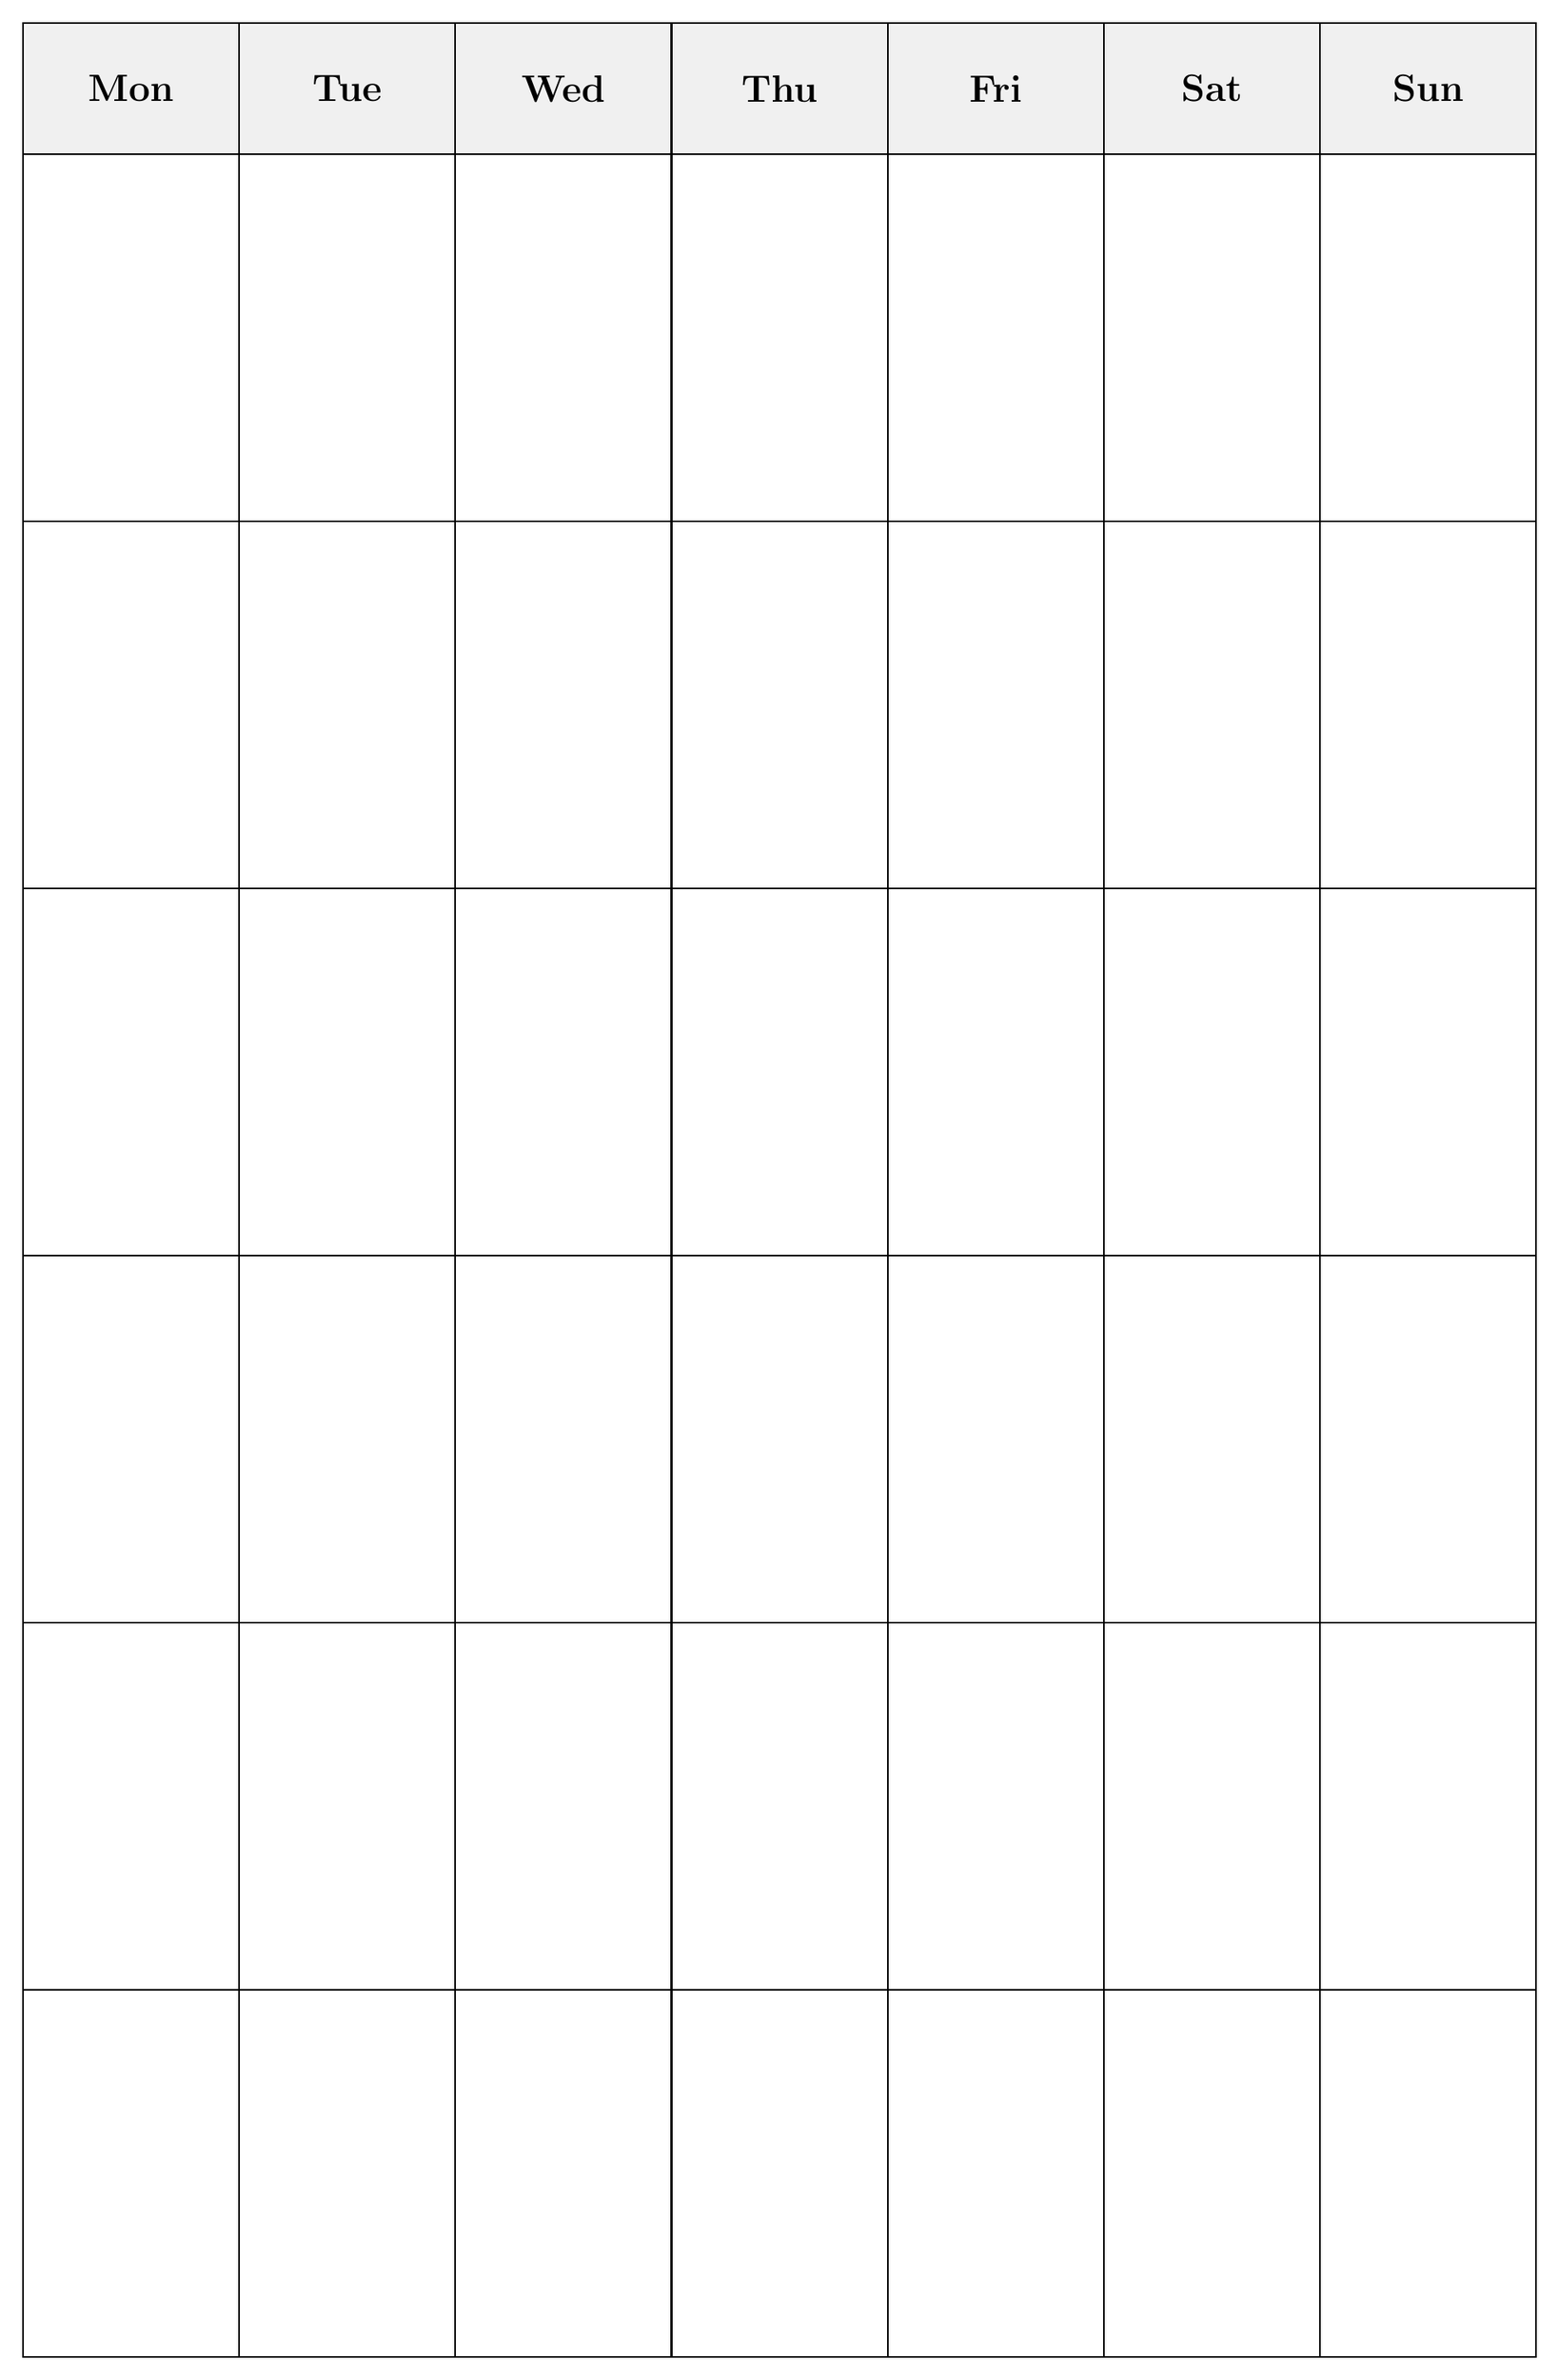
\begin{tikzpicture}[x=1mm,y=1mm]
  % 曜日ヘッダー(月曜始まり)
  \foreach \x/\day in {0/Mon,1/Tue,2/Wed,3/Thu,4/Fri,5/Sat,6/Sun} {
    \pgfmathsetmacro{\xpos}{10+\x*34.57}
    \pgfmathsetmacro{\xposend}{10+(\x+1)*34.57}
    \pgfmathsetmacro{\xcenter}{\xpos+17.285}
    \fill[lightgray] (\xpos,377) rectangle (\xposend,398);
    \draw[thick] (\xpos,377) rectangle (\xposend,398);
    \node[font=\fontsize{16}{20}\selectfont\bfseries] at (\xcenter,387.5) {\day};
  }
  
  % 月曜日を0とするための dowmonday を既に計算
  % カレンダーグリッド描画
  \foreach \row in {0,1,2,3,4,5} {
    \foreach \col in {0,1,2,3,4,5,6} {
      \pgfmathsetmacro{\y}{377-(\row+1)*58.67}
      \pgfmathsetmacro{\yend}{\y+58.67}
      \pgfmathsetmacro{\xpos}{10+\col*34.57}
      \pgfmathsetmacro{\xposend}{10+(\col+1)*34.57}
      \pgfmathtruncatemacro{\cellnum}{\row*7+\col}
      \pgfmathtruncatemacro{\daynum}{\cellnum-\dowmonday+1}
      
      \draw[thick] (\xpos,\y) rectangle (\xposend,\yend);
      
      % 日付表示
      \ifnum\daynum>0
        \ifnum\daynum<\maxdays+1
          \node[anchor=north west,font=\fontsize{14}{16}\selectfont] at ({\xpos+2},{\yend-2}) {
            \hyperlink{daily-2025-\ifnum\monthnum<10 0\fi\monthnum-\ifnum\daynum<10 0\fi\daynum}{\daynum}
          };
        \fi
      \fi
    }
  }
  \end{tikzpicture}
  
  \end{minipage}
  };
  \end{tikzpicture}
  
  \newpage
}

%%% ========================================
%%% PART 2: 54 Weekly Schedules (Week 1-54 of 2025)
%%% ========================================
%%% We'll define week start as Monday of the week that contains Jan 1 shifted by weeks (simple grid)
%%\newcount\weekindex
%%\weekindex=1
%%\foreach \w in {1,...,54} {
%%  \pgfmathtruncatemacro{\weeknum}{\w}
%%  % calculate startJulian = julianJanOne + (weeknum-1)*7 - offsetMonday
%%  \startJulian=\julianJanOne
%%  \advance\startJulian by (\weeknum-1)*7
%%  \advance\startJulian by -\offsetMonday
%%  
%%  % compute end sunday
%%  \juliansunday=\startJulian
%%  \advance\juliansunday by 6
%%  \pgfcalendarjuliantodate{\startJulian}{\tempyear}{\tempmonth}{\tempday}
%%  \pgfcalendarjuliantodate{\juliansunday}{\endyear}{\endmonth}{\endday}
%%  
%%  \hypertarget{weekly-\weeknum}{}
%%  \begin{tikzpicture}[remember picture,overlay]
%%  \node[anchor=north west] at (current page.north west) {
%%  \begin{minipage}[t][452mm][t]{254mm}
%%  
%%  % ヘッダー
%%  \begin{tikzpicture}
%%  \fill[accent!30] (0,0) rectangle (254mm,32mm);
%%  \node[anchor=west,font=\fontsize{36}{40}\selectfont\bfseries] at (10mm,16mm) {Week \weeknum: \monthname{\thetempmonth} \thetempday{} - \monthname{\theendmonth} \theendday};
%%  \node[anchor=east,font=\fontsize{16}{20}\selectfont] at (244mm,16mm) {
%%    \hyperlink{monthly-\thetempmonth}{Monthly} | 
%%    \hyperlink{daily-2025-\ifnum\tempmonth<10 0\fi\thetempmonth-\ifnum\tempday<10 0\fi\thetempday}{Daily}
%%  };
%%  \end{tikzpicture}
%%  
%%  \vspace{5mm}
%%  
%%  % 時間軸付き週間表
%%  \begin{tikzpicture}[x=1mm,y=1mm]
%%  % 曜日ヘッダー(月曜始まり)
%%  \foreach \d in {0,1,2,3,4,5,6} {
%%    % compute current julian for each day
%%    \newcount\currentjulian
%%    \currentjulian=\startJulian
%%    \advance\currentjulian by \d
%%    \newcount\cyear \newcount\cmonth \newcount\cday \newcount\cdow
%%    \pgfcalendarjuliantodate{\currentjulian}{\cyear}{\cmonth}{\cday}
%%    \pgfcalendarjuliantoweekday{\currentjulian}{\cdow}
%%    
%%    \pgfmathsetmacro{\xpos}{10+\d*34.57}
%%    \pgfmathsetmacro{\xposend}{10+(\d+1)*34.57}
%%    \pgfmathsetmacro{\xcenter}{\xpos+17.285}
%%    
%%    \fill[lightgray] (\xpos,380) rectangle (\xposend,396);
%%    \draw[thick] (\xpos,380) rectangle (\xposend,396);
%%    
%%    \node[font=\fontsize{14}{18}\selectfont\bfseries] at (\xcenter,390) {\dayname{\d}};
%%    \node[font=\fontsize{12}{14}\selectfont] at (\xcenter,384) {
%%      \hyperlink{daily-\the\cyear-\ifnum\the\cmonth<10 0\fi\the\cmonth-\ifnum\the\cday<10 0\fi\the\cday}{\the\cmonth/\the\cday}
%%    };
%%  }
%%  
%%  % 時間軸と罫線
%%  \foreach \h in {6,7,8,9,10,11,12,13,14,15,16,17,18,19,20,21,22,23} {
%%    \pgfmathsetmacro{\y}{380-(\h-6)*21.1}
%%    \draw[draw=medgray] (10,\y) -- (252,\y);
%%    \node[anchor=east,font=\fontsize{12}{14}\selectfont] at (9,\y) {\h:00};
%%  }
%%  
%%  % 縦線(曜日の区切り)
%%  \foreach \x in {0,1,2,3,4,5,6,7} {
%%    \pgfmathsetmacro{\xpos}{10+\x*34.57}
%%    \draw[thick] (\xpos,0) -- (\xpos,396);
%%  }
%%  
%%  % 外枠
%%  \draw[very thick] (10,0) rectangle (252,396);
%%  \end{tikzpicture}
%%  
%%  \end{minipage}
%%  };
%%  \end{tikzpicture}
%%  
%%  \newpage
%%}
%%
%%% ========================================
%%% PART 3: 365 Daily Planners
%%% ========================================
%%\foreach \doy in {1,...,365} {
%%  \pgfmathtruncatemacro{\daynum}{\doy}
%%  
%%  % ユリウス日から日付を計算
%%  \pgfcalendardatetojulian{2025-01-01}{\julianday}
%%  \newcount\currentjulian
%%  \currentjulian=\julianday
%%  \advance\currentjulian by \daynum
%%  \advance\currentjulian by -1
%%  
%%  \newcount\cyear \newcount\cmonth \newcount\cday \newcount\cdow \newcount\cweekyear \newcount\cweeknum
%%  \pgfcalendarjuliantodate{\currentjulian}{\cyear}{\cmonth}{\cday}
%%  \pgfcalendarjuliantoweekday{\currentjulian}{\cdow}
%%  \pgfcalendarjuliantoweek{\currentjulian}{\cweekyear}{\cweeknum}
%%  
%%  % 月曜日を0とする
%%  \pgfmathtruncatemacro{\dowmonday}{mod(\cdow+6,7)}
%%  
%%  \hypertarget{daily-\the\cyear-\ifnum\the\cmonth<10 0\fi\the\cmonth-\ifnum\the\cday<10 0\fi\the\cday}{}
%%  \begin{tikzpicture}[remember picture,overlay]
%%  \node[anchor=north west] at (current page.north west) {
%%  \begin{minipage}[t][452mm][t]{254mm}
%%  
%%  % ヘッダー
%%  \begin{tikzpicture}
%%  \fill[accent!30] (0,0) rectangle (254mm,32mm);
%%  \node[anchor=west,font=\fontsize{36}{40}\selectfont\bfseries] at (10mm,16mm) {
%%    \dayfulname{\dowmonday}, \monthname{\the\cmonth} \the\cday
%%  };
%%  \node[anchor=east,font=\fontsize{16}{20}\selectfont] at (244mm,16mm) {
%%    \hyperlink{monthly-\the\cmonth}{Monthly} | \hyperlink{weekly-\the\cweeknum}{Weekly}
%%  };
%%  \end{tikzpicture}
%%  
%%  \vspace{5mm}
%%  
%%  % 左側:時間割
%%  \begin{tikzpicture}[x=1mm,y=1mm]
%%  \draw[very thick] (10,20) rectangle (127,372);
%%  \node[anchor=south,font=\fontsize{16}{20}\selectfont\bfseries] at (68.5,374) {Schedule};
%%  
%%  \foreach \h in {6,7,8,9,10,11,12,13,14,15,16,17,18,19,20,21,22,23} {
%%    \pgfmathsetmacro{\y}{372-(\h-6)*19.56}
%%    \pgfmathsetmacro{\yend}{\y+19.56}
%%    \pgfmathsetmacro{\ycenter}{\y+9.78}
%%    \draw[draw=medgray] (10,\y) -- (127,\y);
%%    \node[anchor=east,font=\fontsize{14}{16}\selectfont] at (23,\ycenter) {\h:00};
%%    \draw[thick] (25,\y) -- (25,\yend);
%%  }
%%  
%%  % 右側:TODO & Notes
%%  \draw[very thick] (132,236) rectangle (244,374);
%%  \node[anchor=south,font=\fontsize{16}{20}\selectfont\bfseries] at (188,376) {TODO};
%%  
%%  \foreach \i in {1,...,12} {
%%    \pgfmathsetmacro{\y}{368-\i*11}
%%    \pgfmathsetmacro{\ycenter}{\y+5.5}
%%    \draw[lightgray] (137,\y) -- (239,\y);
%%    \node[anchor=west,font=\fontsize{12}{14}\selectfont] at (139,\ycenter) {$\square$};
%%  }
%%  
%%  % Notesエリア
%%  \draw[very thick] (132,20) rectangle (244,228);
%%  \node[anchor=south,font=\fontsize{16}{20}\selectfont\bfseries] at (188,230) {Notes};
%%  
%%  \foreach \i in {1,...,18} {
%%    \pgfmathsetmacro{\y}{220-\i*11}
%%    \draw[lightgray] (137,\y) -- (239,\y);
%%  }
%%  \end{tikzpicture}
%%  
%%  \end{minipage}
%%  };
%%  \end{tikzpicture}
%%  
%%  \newpage
%%}

done

\end{document}
